\documentclass[11pt]{article}
\usepackage{geometry}                % See geometry.pdf to learn the layout options. There are lots.
\geometry{letterpaper}                   % ... or a4paper or a5paper or ... 
%\geometry{landscape}                % Activate for for rotated page geometry
%\usepackage[parfill]{parskip}    % Activate to begin paragraphs with an empty line rather than an indent
\usepackage{graphicx}
\usepackage{graphicx}
\usepackage{amssymb}
\usepackage{epstopdf}
\DeclareGraphicsRule{.tif}{png}{.png}{`convert #1 `dirname #1`/`basename #1 .tif`.png}

\newcommand{\Enso}{Ens\={o}}

\title{\Enso}
\author{William R. Cook and Tijs van der Storm}
%\date{}                                           % Activate to display a given date or no date

\begin{document}
\maketitle
%\section{}
%\subsection{}

This paper describes \Enso, a new approach to software 
development. \Enso\ starts from a few simple, but radical
assumptions, from which a complete programming model is then
derived. The basic principles are

information models (cyclic graphs) as data structures

schemas (types) are first-class data that are checked dynamically,
and may also be derived/computed dynamically

generic operations, guided by meta-data, include equality, difference,
merge, parse, and rendering. Operations use cyclic maps to transform 
cyclic data.









\begin{itemize}

\item \Enso\ represents data as collections of entities with attributes
and connected into a graph via relationships. 
Data is not broken into atomic pieces (objects, records, or tuples), but is
instead managed holistically as cyclic data structures.

\item Data is described by schemas, which have 
metadata about structure, behavior, and intent.

\item Generalized grammars describe how
data is presented in a variety of formats, including
text, diagrams, GUIs, and web pages.
Most presentations are bi-directional.

\item Interactive presentation structures define legal editing operations
to insert, delete, and modify the original structure.
Data binding is implicit and automatic.

\item Generic operations, guided by metadata, perform
complex transformations on arbitrary structures.

\item Transformation on cyclic structures are natural.
The system generalizes attribute grammars.

\item Schemas and presentations are also data, and 
are frequently generated, transformed, and merged.

\item Everything, including the fundamental schemas
in the system, is extensible.

\item Change is encouraged and managed. Changes to
schemas are represented as instances of delta schemas.
Schema changes guide instance upgrades.

\item Everything, including schemas, grammars and
transformations, can be composed and mixed together
to support extreme reuse and feature modularity

\item The entire system is dynamic, but tightly 
constrained by the dynamic metadata. We have 
demonstrated that partial evaluation and supercompilation 
can specialize generic operations to create efficient 
code.

\item Serialization is avoided. Instead every kind of 
data is presented in a language, so that it can be 
versioned and managed.

\item There is a natural mapping to relational databases,
especially since bulk operations on information structures
is fundamental to \Enso. We view query results as 
mini-databases, not as single tables. 

\end{itemize}

\subsection{Relationship to Other Approaches}

\Enso\ data is based on traditional 
entity-relationship (ER) models \cite{FOO},
which are also known as information models. 
ER models were the basis for class diagrams in UML.

In contrast to
object-oriented programming, \Enso\ is focused on holistic
object graphs, rather than individual objects. \Enso\ 
does allow data to include some behavior, for example constraints
and computed fields, but \Enso\ does not associated methods
with data objects.

In contrast to
most theories of functional programming, \Enso\ is based on
coalgebraic signatures rather than algebraic ones. In practice
this means that \Enso\ structures are cyclic graphs rather than
trees. Lazy functional languages can also represent cyclic 
structures, but the cycles are not observable.

\Enso\ supports controlled imperative effects. Objects are
mutable during construction or modification, while the data may be in an
inconstent state, but before it can be used it must be validated
and locked from further changes. This is similar to a transaction.


\Enso\ data is 

\subsection{Data}

\Enso\ represents all data via graphs whose structure is defined
by a form of entity-relationship model, called a \textit{schema}. 
\Enso\ shifts focus away from individual pieces of data, to focus instead
on semantically integrated collections of data. 

An \Enso\ data structure is analogous to an information model,
a relational database, an object model without methods, or a coalgebra.
While it is easy to create specialized data modeling notations
in \Enso, the standard information model has the following properties:

\subsection{Presentation}






as cyclic graphs, where
nodes are categories into types that have 
consistent attributes and edges are labeled.

All data is represented as cyclic graphs of 


"information model": 
"relational database": the nodes of the graph are
rows of the tables. Foreign keys 

Data is represented as 



This example converts schemas into constructor grammars
\begin{verbatim}
grammar NAME:sym
   CLASSES:
     rule NAME:sym = 
        (SUBTYPES: { NAME:sym "|") "|" @"!SUBTYPES.empty?")?
         [NAME:sym] NAME:str "{" 
            FIELDS: { (NAME:str ":" (NAME:sym): (
                 "[" { TYPE.NAME:sym^ "," } "]"   @"MANY=true"
               | TYPE.NAME:sym^ ?                  @"OPTIONAL=true"
               | TYPE.NAME:sym^
               )) ";" }
             "}"
\end{verbatim}


\section{Requirements for a programming language}

The programming model is based on cyclic graphs.
Graphs are kept distinct from each other. That is,
each graph is considered a self-contained
artifact, without links or pointers to other graphs.

A natural way to create such graphs is with 
imperative effects.

This potentially requires more copying of data
than would be the case in tree-based representations.

To modify graphs, place-holder objects are useful,
as is the ability to "become" another object.

\subsection{Simple reflection}

Fields can be created dynamically and accessed with
"." notation or reflective access.

\begin{verbatim}
o.foo   == o.get("foo")
\end{verbatim}

Assignment to fields can be overriden
\begin{verbatim}
   o.bar = 3   ==> o.set("bar", 3)
\end{verbatim}



\section{QuadModel}

\section{Todos}

* merging schemas and grammars. Need a merge operation. Based on identification/unification

* Finalize on objects, that checks required fields, seals from changes, run invariants
   
* removing "key" from grammar

* fix pretty printing 

* GUIs

* fixedpoint cyclic map





* checked model-objects (with correct inverses and type checking)
* derivative parsers?
* other kind of parser?
* executable UML?
* graphical editors?
    (does Ruby have graphics binding?)
* database mapping?
* WebDSL mini-language




\begin{figure}[htbp]
\begin{center}
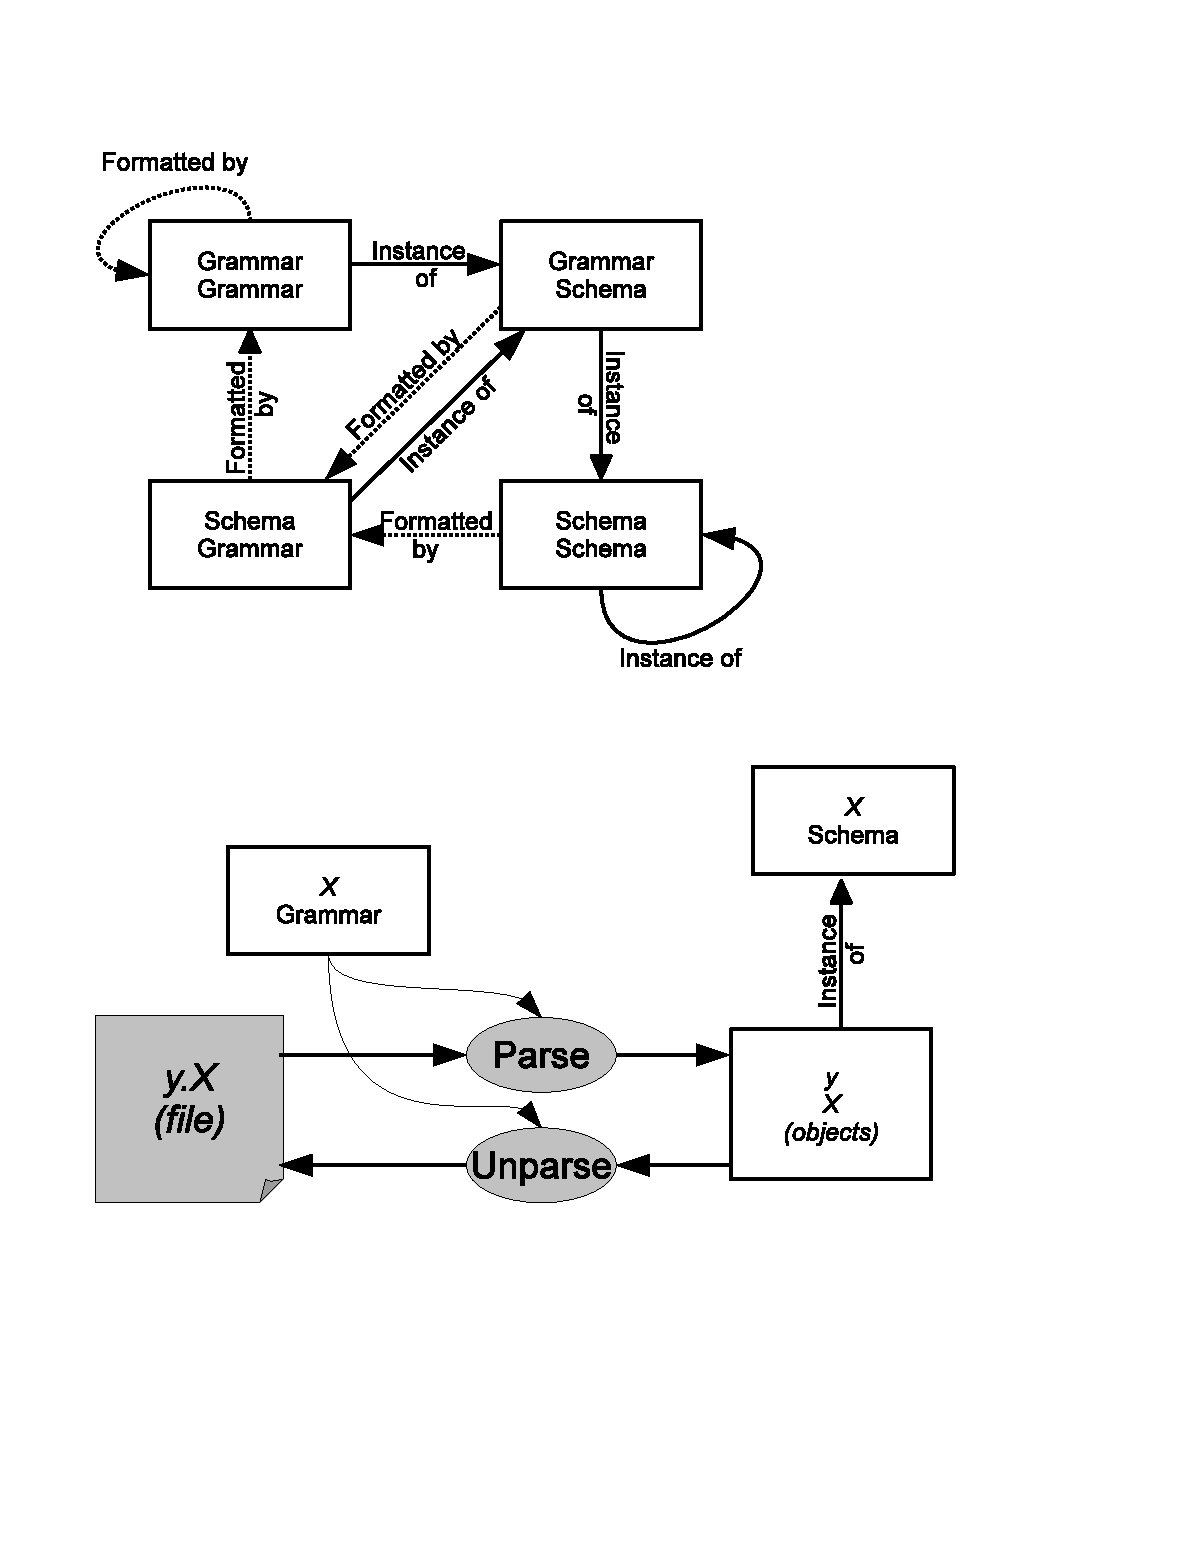
\includegraphics[scale=0.8]{QuadModel.eps}
\caption{{\bf default}}
\label{default}
\end{center}
\end{figure}



\end{document}  